


%----------------------------------
\chapter{Introduction}\label{ch:Relativeintro}
%----------------------------------

\section{Purpose and Objectives of the \RelativeDescT}
%%%%%%%%%%%%%%%%%%%%%%%%%%%%%%%%%%%%%%%%%%%%%%%%%%%%%%%%%%%%%%%%%%%%%%%%%%%%%%%%%
%
% Purpose:  Introduction for the Relative model.
%
% 
%
%%%%%%%%%%%%%%%%%%%%%%%%%%%%%%%%%%%%%%%%%%%%%%%%%%%%%%%%%%%%%%%%%%%%%%%%%%%%%%%%


%\section{Purpose and Objectives of \RelativeDesc}
% Incorporate the intro paragraph that used to begin this Chapter here. 
% This is location of the true introduction where you explain what this model 
% does.
The \RelativeDesc\ allows the state of one reference frame (e.g. the body reference frame of a vehicle) to be expressed relative to any other reference frame (e.g., the LVLH reference frame of another vehicle). As of JEOD version 3.4, it is no longer required that one of the reference frames be associated with a DynBody; the relative state can now be calculated between any two arbitrary frames in the simulation.

















%----------------------------------
\chapter{Product Requirements}\label{ch:Relativereqt}
%----------------------------------


%%%%%%%%%%%%%%%%%%%%%%%%%%%%%%%%%%%%%%%%%%%%%%%%%%%%%%%%%%%%%%%%%%%%%%%%%%%%%%%%%
%
% Purpose:  requirements for the Relative model
%
% 
%
%%%%%%%%%%%%%%%%%%%%%%%%%%%%%%%%%%%%%%%%%%%%%%%%%%%%%%%%%%%%%%%%%%%%%%%%%%%%%%%%

% add text here to describe general model requirements
% text is of the form:
\requirement{Relative representation}
\label{reqt:Relative}
\begin{description}
  \item[Requirement:]\ \newline
     The Relative Derived State will provide the capability for expressing the state of one reference frame relative to some other reference frame in a specified frame of reference.
  \item[Rationale:]\ \newline
     Capability from JEOD 1.5.
  \item[Verification:]\ \newline
     Inspection, unit test, integrated test by proxy.
\end{description}

\section{Requirements Traceability}

\begin{longtable}[c]{||p{3.5in}|p{3.5in}|}
\caption{Requirements Traceability} \\[6pt]
\hline
{\bf Requirement} & {\bf Inspection and Testing} \\ 
\hline \hline
\endhead
\ref{reqt:Relative} - Relative State Representation &
  Insp.~\ref{inspect:Relative} \\ 
  &
  Test~\ref{test:Relative} \\ \hline

\end{longtable}




%----------------------------------
\chapter{Product Specification}\label{ch:Relativespec}
%----------------------------------

\section{Conceptual Design}
%%%%%%%%%%%%%%%%%%%%%%%%%%%%%%%%%%%%%%%%%%%%%%%%%%%%%%%%%%%%%%%%%%%%%%%%%%%%%%%%%
%
% Purpose:  Conceptual part of Product Spec for the Relative model
%
% 
%
%%%%%%%%%%%%%%%%%%%%%%%%%%%%%%%%%%%%%%%%%%%%%%%%%%%%%%%%%%%%%%%%%%%%%%%%%%%%%%%%


%\section{Conceptual Design}

The \RelativeDesc\ provides the state of one vehicle with respect to some other reference frame (often associated with another vehicle, but not necessarily so).  The two reference frames (the vehicle's reference frame and the other reference frame) are labeled \textit{subject} and \textit{target}.  This model is sufficiently flexible to represent the state of either reference frame with respect to the other.  As of version 3.4, the \textit{subject} frame no longer must be associated with a Dynamic Body, but can be any arbitrary frame in the simulation.  However, the model is fully backwards compatible to the previous usage when it was required to be associated with a Dynamic Body. The \textit{target} never had the Dynamic Body restriction. The original intent was that the subject of the relative state calculation be a vehicle, while the target could be a planet, or some defined point unassociated with any mass, though in actuality the calculation is the same regardless of the nature of the reference frame's owning point or model. The updated capability reflects this.

When expressing the state of some frame, \textit{A} with respect to some other frame, \textit{B}, the tranlational position and velocity are expressed in frame \textit{B}, while the angular velocity is expressed in frame \textit{A}; the angular position (expressed as a quaternion or transformation matrix) is frame-independent.

As a simple example, consider two reference frames, \textit{S} and \textit{S'}.  Suppose that \textit{S'} is moving with some velocity \textit{u} along the x-axis of reference frame \textit{S}, and has its origin momentarily located at $(x_0,y_0)$  Consider further that \textit{S'} is rotated by ninety degrees about the z-axis from \textit{S}, so that $x' = y,  y' = -x, z' = z$.  An illustration is shown in Figure~\ref{fig:relstatereforient}.

\begin{figure}[ht]
\begin{center}
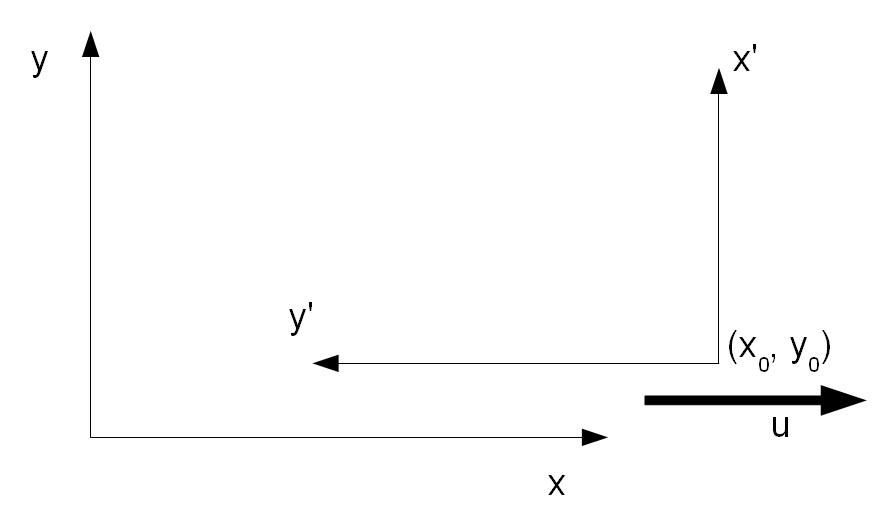
\includegraphics[width=3.5in]{figures/rel_state_ref_orient.jpg}
\caption{The momentary positions, velocity, and orientation of frames \textit{S} and \textit{S'}}
\label{fig:relstatereforient}
\end{center}
\end{figure}

There are four ways of expressing this relation:  the state of \textit{S'} can be expressed with respect to \textit{S}, or \textit{S} with respect to \textit{S'}; for each case, the result could be expressed in \textit{S} or in \textit{S'}.  In this example, the state of  \textit{S'} with respect to \textit{S}, can be represented as 

\begin{align*}
\vec x_{S'|S:S} & = (x_0, y_0) \\ 
\vec v_{S'|S:S} & = (u,0)\\
\vec x_{S'|S:S'} & = (y_0, -x_0) \\
\vec v_{S'|S:S'} & = (0,-u)
\end{align*}

where $ \vec x_{A|B:C}$ is the position of A with respect to B, expressed in C.

Similarly, the state of  \textit{S} with respect to \textit{S'}, can be represented as 

\begin{align*}
\vec x_{S\_S':S} & = (-x_0, -y_0) \\
\vec v_{S\_S':S} & = (-u,0)\\
\vec x_{S\_S':S'} & = (-y_0, x_0)\\
\vec v_{S\_S':S'} & = (0,u)
\end{align*}

Thus, the relative position (or velocity) could be described in four ways, using just these two frames.  Of these four representations, this model can provide $\vec x_{S'|S:S}$ and $\vec x_{S\_S':S'}$.

To make the system completely generic, the usage of \textit{subject} and \textit{target} are, for the most part, just names.  The \RelativeDesc\ will calculate the state of either with respect to the other.  Hence, in the example above, S and S' can be interchangeably identified as \textit{subject} and \textit{target}.  Again, the only restriction on assigning the \textit{subject} and \textit{target} is that the \textit{subject} must be associated with a Dynamic Body.

The user must specify three quantities:
\begin{itemize}
\item{Subject reference frame (by name)}
\item{Target reference frame (by name)}
\item{Sense in which to interpret the request}
\end{itemize}

the latter item in this list can be one of the two values described above:
\begin{itemize}
\item{Subject with respect to Target, expressed in Target (ComputeSubjectStateinTarget)}
\item{Target with respect to Subject, expressed in Subject (ComputeTargetStateinSubject)}
\end{itemize}

Note that this description is intended to convey information on the translational state only.  The angular velocity of the Subject frame will be expressed in the Subject frame, and the angular velocity of the Target frame will be expressed in the target frame.  The expression of the relative orientations of the two frames is frame independent.

%\section{Mathematical Formulations}
%%%%%%%%%%%%%%%%%%%%%%%%%%%%%%%%%%%%%%%%%%%%%%%%%%%%%%%%%%%%%%%%%%%%%%%%%%%%%%%%%
%
% Purpose:  Mathematical Formulation part of Product Spec for the Relative model
%
% 
%
%%%%%%%%%%%%%%%%%%%%%%%%%%%%%%%%%%%%%%%%%%%%%%%%%%%%%%%%%%%%%%%%%%%%%%%%%%%%%%%%

\section{Mathematical Formulations}

The mathematical formulation for calculating the \RelativeDesc\ is entirely incorporated into the Reference Frames model (see \href{file:\JEODHOME/models/utils/ref_frames/docs/ref_frames.pdf}{\em Reference Frames}~\cite{dynenv:REFFRAMES}).
%\section{Detailed Design}

%%%%%%%%%%%%%%%%%%%%%%%%%%%%%%%%%%%%%%%%%%%%%%%%%%%%%%%%%%%%%%%%%%%%%%%%%%%%%%%%%
%
% Purpose:  Detailed part of Product Spec for the Relative model
%
% 
%
%%%%%%%%%%%%%%%%%%%%%%%%%%%%%%%%%%%%%%%%%%%%%%%%%%%%%%%%%%%%%%%%%%%%%%%%%%%%%%%%

\section{Detailed Design}
\label{sec:relativedetail}
See the \href{file:refman.pdf}{Reference Manual}\cite{derivedstatebib:ReferenceManual} for a summary of member data and member methods for all classes.  

\subsection{Process Architecture}
The architecture for the \RelativeDesc\ is trivial, comprising methods that are operationally independent.

\subsection{Functional Design}
This section describes the functional operation of the methods in each class.


The \RelativeDesc\ contains only one class:

\begin{itemize}
\classitem{RelativeDerivedState}
\label{ref:RelativeDerivedState}
\textref{DerivedState}{ref:DerivedState}

This contains only the methods \textit{initialize} and \textit{update}:
\begin{enumerate}
\funcitem{initialize}
The initialization process comprises the following steps:
\begin{enumerate}
\item{} The generic DerivedState initialization routine is called to assign the \textit{subject} value, and establish the naming convention for the state identifier.  Note - this is based on the \textit{subject} name, not on the \textit{target} name.  The user may wish to consider this in determining which object to associate as target, and which to associate as subject.
\item{} Ensures that the \textit{subject\_frame} and \textit{target\_frame} are well-defined.
\item{} The registry of active bodies, maintained by the Dynamics Manager (see \href{file:\JEODHOME/models/dynamics/dyn_manager/docs/dyn_manager.pdf}{\em Dynamics Manager Documentation}~\cite{dynenv:DYNMANAGER}) is updated to ensure that the \textit{target\_frame} is being updated, if necessary.
\end{enumerate}

\funcitem{update}
The variable \textit{direction\_sense} can be set to one of two values:
\begin{enumerate}
\item{ComputeSubjectStateinTarget}
\item{ComputeTargetStateinSubject}
\end{enumerate}

The appropriate call is made to the appropriate reference frame's \textit{calculate\_relative\_state} method, using the other reference frame as an argument (e.g., for ComputeSubjectStateinTarget, we are looking for the state of \textit{subject} with respect to \textit{target}, so the subject-frame's method would be called, using the target frame as an argument).


\end{enumerate}
\end{itemize}





\chapter{User's Guide}\label{ch:Relativeuser}
%----------------------------------
The Analysis section of the User's Guide is intended primarily for
users of pre-existing simulations.  
It contains: 
\begin{itemize}
\item A description of how to modify \RelativeDesc\ variables after
the simulation
has compiled, including an in-depth discussion of the input file,
\item An overview of how to interpret (but not edit) the S\_define
file,
\item A sample of some of the typical variables that may be logged.
\end{itemize}

The Integration section of the User's Guide is intended for simulation
developers.
It describes the necessary configuration of the \RelativeDesc\
within an
S\_define file, and the creation of standard run directories.  The
latter
component assumes a thorough understanding of the preceding Analysis
section of the user guide.
Where applicable, the user may be directed to selected portions of
Product Specification (Chapter \ref{ch:Relativespec}).

The Extension section of the User's Guide is intended primarily for
developers
needing to extend the capability of the \RelativeDesc.  Such users
should have a
thorough understanding of how the model is used in the preceding
Integration section, and of the model
specification (described in Chapter \ref{ch:Relativespec}).


\section{Analysis}
%%%%%%%%%%%%%%%%%%%%%%%%%%%%%%%%%%%%%%%%%%%%%%%%%%%%%%%%%%%%%%%%%%%%%%%%%%%%%%%%%
%
% Purpose:  Analysis part of User's Guide for the Relative model
%
% 
%
%%%%%%%%%%%%%%%%%%%%%%%%%%%%%%%%%%%%%%%%%%%%%%%%%%%%%%%%%%%%%%%%%%%%%%%%%%%%%%%%

% \section{Analysis}

\label{sec:relativeuseranalysis}

\subsection{Identifying the \RelativeDescT}
If Relative States have been included in the simulation, there will be an instance of \textit{RelativeDerivedState} located in the S\_define file.  This would typically be found in either the vehicle object, or a separate relative-state object.  There should be an accompanying call to both an initialization routine and an update function.  The \textit{target\_frame} and \textit{subject\_frame} are defined elsewhere, possibly in the input file.

Example:
\begin{verbatim}
sim_object{
dynamics/derived_state:    RelativeDerivedState example_of_rel_der_state;

(initialization) dynamics/derived_state:
example_of_rel_state_object.example_of_rel_der_state.initialize (
    Inout DynBody &      subject_body = vehicle_1.dyn_body,
    Inout DynManager &   dyn_manager  = manager_object.dyn_manager);
    
{environment} dynamics/derived_state:
example_of_rel_state_object.example_of_rel_der_state.update ( )

} example_of_rel_state_object;
\end{verbatim}

Then the input file may have entries comparable to:
\begin{verbatim}
example_of_rel_state_object.example_of_rel_der_state.subject_frame_name = 
                                                 "vehicle_1.composite_body";
example_of_rel_state_object.example_of_rel_der_state.target_frame_name = 
                                                 "vehicle_2.Earth.lvlh";
example_of_rel_state_object.example_of_rel_der_state.direction_sense = 
                              RelativeDerivedState::ComputeSubjectStateinTarget;
\end{verbatim}

(In this case, the relative state provides the state of \textit{vehicle\_1} in the Earth-based LVLH frame associated with \textit{vehicle\_2}.  Note that there are many variations on this concept, so the analyst should not be surprised if entries are significantly different from this example).

As of JEOD version 3.4, it is no longer required that a relative state be associated with a vehicle object. Thus, it can be used to calculate the state between any two arbitrary frames in the simulation. To use it in this manor, one needs only to invoke the initialization routine that does not take a \textit{subject\_body} as input:

\begin{verbatim}
(initialization) dynamics/derived_state:
example_of_rel_state_object.example_of_rel_der_state.initialize (
    Inout DynManager &   dyn_manager  = manager_object.dyn_manager);
\end{verbatim}

All other usage remains the same.

\subsection{Editing the \RelativeDescT}
There is very little to edit in the \RelativeDesc.  Changing the \textit{direction\_sense} is trivial (see section \textref{Detailed Design}{sec:relativedetail} for options).  Changing the \textit{subject\_frame} and \textit{target\_frame} may produce unintended consequences, and should not be attempted at this level; see the \textref{Integration}{sec:relativeintegration} for details on setting up a relative state calculation.


\subsection{Output Data}
The output available from this model is a complete 12-vector state description.

The translational component of the state is accessible as
\begin{verbatim}
example_of_rel_state_object.example_of_rel_der_state.rel_state.trans.position
example_of_rel_state_object.example_of_rel_der_state.rel_state.trans.velocity
\end{verbatim}
The rotational state can be output as either quaternion or transformation matrix, with velocity as either an angular velocity vector, or an angular velocity magnitude and unit vector.  See the documentation on \textit{RefFrameState} in the \href{file:\JEODHOME/models/utils/ref_frames/docs/ref_frames.pdf}{RefFrame document}~\cite{dynenv:REFFRAMES} for details.


%\section{Integration}
%%%%%%%%%%%%%%%%%%%%%%%%%%%%%%%%%%%%%%%%%%%%%%%%%%%%%%%%%%%%%%%%%%%%%%%%%%%%%%%%%
%
% Purpose:  Integration part of User's Guide for the Relative model
%
% 
%
%%%%%%%%%%%%%%%%%%%%%%%%%%%%%%%%%%%%%%%%%%%%%%%%%%%%%%%%%%%%%%%%%%%%%%%%%%%%%%%%

 \section{Integration}
\label{sec:relativeintegration}

Including the \RelativeDesc\ into the simulation requires some knowledge of other reference frames and derived states.

 \subsection{Generating the S\_define}

Conventional practice would add the \RelativeDesc\ to a separate relative-state object at the end of the S\_define file.  It is also possible to add the relative state to a specific vehicle, but care must be taken to ensure that the target frame has been fully updated before the relative state is called.  For example, if the relative state is to be between two vehicles, \textit{A} and \textit{B} (suppose \textit{A} is the \textit{subject}, and \textit{B} the \textit{target}), then the relative state must be generated after object \textit{B}, and the particular reference frame of interest associated with \textit{B}, are both updated.  A simple solution to this is to either place the relative state calculation at the end of the simulation, or to prioritize the call to update the relative state such that is is processed after that of \textit{B}.  There is no internal check that this ordering is achieved, the responsibility for ensuring this lies entirely on the Integrator.

The instance of \textit{RelativeDerivedState} needs to be defined, the model initialized, and a routine update scheduled.  A simple example of how this may look is found in the \textref{Analysis}{sec:relativeuseranalysis} section.  Simple example simulations are found in the verification simulations for the \textref{\NEDDesc}{ch:NEDivv} and the \textref{\LVLHDesc}{ch:LVLHivv} released with \JEODid.  For more complicated setups, where there are multiple relative states defined, it is strongly recommended that all relative states be put together into one relative state object, and grouped under the Relative Kinematics manager.  This manager handles all of the relative states together after all of the individual frames have been evaluated, and avoids the need to make a separate call from the S\_define for each individual state.  See the \href{file:\JEODHOME/models/dynamics/rel\_kin/docs/rel\_kin.pdf}{Relative Kinematics}~\cite{dynenv:RELKIN} document for details.

\subsection{Generating the Input File}
The input file (or Modified Data file) must contain the names of the \textit{subject\_frame} (\textit{subject\_frame\_name}) and \textit{target\_frame} (\textit{target\_frame\_name}), as well as the \textit{direction\_sense} for each instance of a RelativeDerivedState.  The \textit{subject\_body} is defined elsewhere, as it is passed into the initialization routine from the S\_define.  The \textit{subject\_body} so passed into the initialization routine must include a reference frame with a name that matches the \textit{subject\_frame\_name}, or the initialization routine will fail.  See the \href{file:\JEODHOME/models/utils/ref\_frames/docs/ref\_frames.pdf}{Reference Frames}~\cite{dynenv:REFFRAMES} documentation for more details on the convention for naming the reference frames.

See the \textref{Analysis}{sec:relativeuseranalysis} section for an example of how the input data may appear.

\subsection{Logging the Data}
There are multiple variables available for output, to represent the 12-vector state description.  The most commonly used are the relative position and velocity, which are logged by adding the following lines to the list of logging data:
\begin{verbatim}
"example_of_rel_state_object.example_of_rel_der_state.rel_state.trans.position[0-2]",
"example_of_rel_state_object.example_of_rel_der_state.rel_state.trans.velocity[0-2]",
\end{verbatim}

The rotational state has some flexibility in its representation.  The angular position can be accessed through a quaternion or transformation matrix representation, e.g.
\begin{verbatim}
"example_of_rel_state_object.example_of_rel_der_state.rel_state.rot.T_parent_this[0][0-2]",
"example_of_rel_state_object.example_of_rel_der_state.rel_state.rot.T_parent_this[1][0-2]",
"example_of_rel_state_object.example_of_rel_der_state.rel_state.rot.T_parent_this[2][0-2]",
\end{verbatim}

and the angular rates can be accessed through the angular velocity vector, or with a magnitude and unit vector representation, e.g.
\begin{verbatim}
"example_of_rel_state_object.example_of_rel_der_state.rel_state.rot.ang_vel_this[0-2]",
\end{verbatim}


%\section{Extension}
%%%%%%%%%%%%%%%%%%%%%%%%%%%%%%%%%%%%%%%%%%%%%%%%%%%%%%%%%%%%%%%%%%%%%%%%%%%%%%%%%
%
% Purpose:  Extension part of User's Guide for the Relative model
%
% 
%
%%%%%%%%%%%%%%%%%%%%%%%%%%%%%%%%%%%%%%%%%%%%%%%%%%%%%%%%%%%%%%%%%%%%%%%%%%%%%%%%

 \section{Extension}

The \RelativeDesc\ is not intended to be extensible at this time.  An obvious conceptual extension would be the ability to state the frame used to express the state of frame \textit{A} with respect to frame \textit{B}, as opposed to the current capability which dictates the expression frame (e.g. one could wish to express the relative position of frame \textit{A} with respect to frame \textit{B} in frame \textit{A}, or in a third frame, frame \textit{C}, but neither capability is currently available).  However, great care should be taken if this is attempted, due to the nature of the inherent paradigm of the RefFrameState.

 The \RelativeDesc\ takes advantage of the RefFrameState object to describe the state.  It is assumed that the RefFrameState (of frame \textit{A} relative to frame \textit{B}) has the following interpretations:
 \begin{itemize}
  \item Position: expresssed in frame \textit{B}.
  \item Translational velocity: expresssed in frame \textit{B}.
  \item Rotational velocity: expresssed in frame \textit{A}.
 \end{itemize}
 The RefFrameState contains not only those state elements (if it did, the extension would be a trivial transformation), but also provides the methods to manipulate them.  Changing the paradigm by transforming the output data values will make the output inconsistent with the class that represents it, and will invalidate those methods.  However, the output will still be a RefFrameState, so those invalid methods will still be applicable, however inappropriately;  peculiar and unexpected behavior will likely result.  So, while the \RelativeDesc\ can be easily extended conceptually, the implementation of that extension is far beyond the scope of this document.  The capability to provide these extensions is currently under review for future releases.
 


%----------------------------------
\chapter{Verification and
Validation}\label{ch:Relativeivv}
%----------------------------------

\section{Verification}
%%%%%%%%%%%%%%%%%%%%%%%%%%%%%%%%%%%%%%%%%%%%%%%%%%%%%%%%%%%%%%%%%%%%%%%%%%%%%%%%%
%
% Purpose:  Verification part of V&V for the Relative model
%
% 
%
%%%%%%%%%%%%%%%%%%%%%%%%%%%%%%%%%%%%%%%%%%%%%%%%%%%%%%%%%%%%%%%%%%%%%%%%%%%%%%%%

% \section{Verification}

%%% code imported from old template structure
\subsection{Inspection of Behavior in Integrated Testing}
\inspection{Inspection of LVLH and NED Verification Simulations}\label{inspect:Relative}
  The verification of the integrated behavior of the \RelativeDesc\ is performed by proxy in the verification of the \textref{\NEDDesc}{ch:NEDivv} and \textref{\LVLHDesc}{ch:LVLHivv}.  The performance of the simulations in these verification tests indicates that the \RelativeDesc\ is performing as expected at a crude, conceptual level (comparison against analytical results was not performed in this case). This result partially satisfies requirement~\ref{reqt:Relative}.  Requirement~\ref{reqt:Relative} is fully satisfied with the demonstration of performance against analytical results; this demonstration is provided in Test~\ref{test:Relative}. 


\subsection{Analytical Verification of Comprehensive Behavior in Unit Testing}

\test{Analytical Verification of \RelativeDescT\ Output Data for Multiple Scenarios}\label{test:Relative}

\begin{description}
\item[Purpose:]
To demonstrate that the data output by the \RelativeDesc\ provides accurate relative state information in simple, analytical  situations.

\item[Requirements:]
Satisfactory conclusion of this test partially satisfies requirement~\ref{reqt:Relative}.  Requirement~\ref{reqt:Relative} is fully satisfied with the additional demonstration of satisfactory performance within integrated testing; this demonstration is conducted at Inspection~\ref{inspect:Relative}.

\item[Procedure:]
A simulation was developed containing two vehicles in empty space.  Each vehicle
contained one vehicle-point.  Tests were run with the vehicles initialized in
various relative states, and the relative states between the points were
examined.  The state outputs were provided as the relative state of:
\begin{itemize}
 \item A with respect to B, expressed in reference frame B
 \item B with respect to A, expressed in reference frame A
\end{itemize}

\textbf{Notation:}
\begin{itemize}
\item 
Vectors are expressed numerically as a set of three values enclosed in square braces ($[x,y,z]$).
Subscripts on a vector denote the reference frame in which the values are expressed (i.e. which x,y,z axes are being used).
The subscripts used in this section are:
\begin{itemize}
 \item I - inertial
 \item SA - structural of vehicle A
 \item SB - structural of vehicle B
 \item PA - point frame of vehicle A
 \item PB - point frame of vehicle B 
\end{itemize}
\item Position, velocity and angular velocity are symbolically represented by:
\begin{itemize}
 \item $\vec x$ Position.
 \item $\vec v$ Translational velocity.
 \item $\vec \omega$ Rotational velocity.
\end{itemize}
\item Subscripts on the symbolic vector values are to be interpreted as follows ($P$, $Q$, and $R$ are used here as representatives of the frames used in this section):
\begin{itemize}
 \item $\vec x_{P}$ Position of frame $P$ (reference taken from context).
 \item $\vec x_{P|Q}$ Position of frame $P$ with respect to frame $Q$ (expression frame taken from context).
 \item $\vec x_{P|Q:R}$ Position of frame $P$ with respect to frame $Q$, expressed in frame $R$.
\end{itemize}
\item Conventionally,
\begin{itemize}
 \item $\vec x_{P|Q}$ is expressed in frame Q.
 \item $\vec v_{P|Q}$ is expressed in frame Q.
 \item $\vec \omega_{P|Q}$ is expressed in frame P.
\end{itemize}
\end{itemize}



The vehicles were configured as shown in Figure~\ref{fig:Relative_config}.  For
both vehicles, the respective structure and body frames are equivalent; the body frame will 
therefore not be mentioned again in this section.  

Vehicle B
is initially located such that $\vec x_{SB|I} = [0,0,0]_I$, with frame \textit{SB} aligned
with frame \textit{I}.  


Point B (the vehicle point on Vehicle B) is located at \newline
$\vec x_{PB|SB} = [1,0,0]_{SB}$ (initial conditions, $\vec x_{PB|I} = [1,0,0]_I$).
Frame \textit{PB} is initially rotated by -90 degrees
 about the z-axis with respect to frame \textit{SB}.

 Vehicle A is initially located such that $\vec x_{SA|I} = [10, 0, 0]_I$.  Its structural
 reference frame (\textit{SA}) is oriented with a +90 degree rotation about the z-axis from
 frame \textit{I}.  
 
 Frame \textit{PA}, associated with Point A,
 is located such that $\vec x_{PA|SA} = [1, 0, 0]_{SA}$ (initial conditions, $\vec x_{PA|I} =[10,1,0]_I$).
 It has a +90 degree rotation about the z-axis with respect to frame \textit{SA}.

 The dynamic states, where applicable, of the two vehicles are initialized such that:
 \begin{itemize}
   \item $\vec v_{SA|I} = [2 , 1 , 0 ]_I = [-2 , -1 , 0]_{PA}$
   \item $\vec \omega_{SA|I} = [0 , 9 , 0]_{SA}\ deg\ s^{-1} = [-9 ,
   0 , 0]_I\ deg\ s^{-1} = [9 , 0 , 0]_PA\ deg\ s^{-1}$
   \item $\vec v_{SB|I} = [0 , 0 , 1]_I$
   \item $\vec \omega_{SB|I} = [0 , 0 , 4.5]_I\ deg\ s^{-1}$ (same value in frames I,
   SB, PB).
 \end{itemize}

\begin{figure}[!ht]
 \begin{center}
  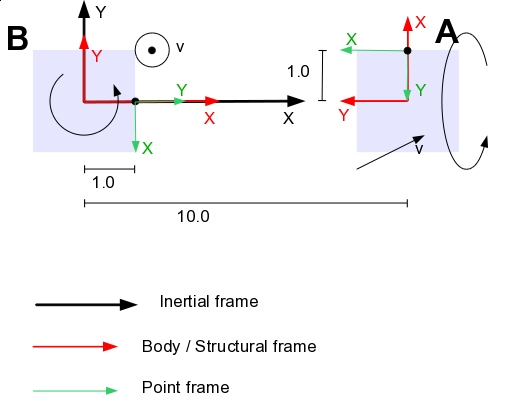
\includegraphics[width=80mm]{figures/relative_config.png}
  \caption{The configuration of the two vehicles and their respective reference frames.} 
  \label{fig:Relative_config}
 \end{center}
\end{figure}


Several simulation setups were considered, gradually increasing in complexity.

First, the rotational states were turned off, and only the effects of 
relative translational motion studied -- first one at a time, then both moving
together.
Then, the translational motion was zeroed, and only the effect of
relative rotational motion considered -- first one at a time, then both
together.
Finally, the situation in which both vehicles had translational and rotational
motion was considered.

\begin{enumerate}
 \item RUN\_no\_rot\_A\_trans
 \item RUN\_no\_rot\_B\_trans
 \item RUN\_no\_rot\_AB\_trans
 \item RUN\_A\_rot\_no\_trans 
 \item RUN\_B\_rot\_no\_trans
 \item RUN\_AB\_rot\_no\_trans  
 \item RUN\_AB\_rot\_AB\_trans  
\end{enumerate}

\item[Predictions:]



\begin{enumerate}
 \item RUN\_no\_rot\_A\_trans \newline
   With no rotation, the relative states are straightforward.  In this case, only vehicle A is moving.
   \begin{itemize}
    \item $\vec x_{PA|PB} = [(-1 - t), (9 + 2t) , 0]_{PB}$
    \item $\vec v_{PA|PB} = [-1 , 2 , 0]_{PB}$
    \item $\vec \omega_{PA|PB} = [0 , 0 , 0]_{PA}$
    \item $\vec x_{PB|PA} = [(9 + 2t) , (1 + t) , 0]_{PA}$
    \item $\vec v_{PB|PA} = [2 , 1 , 0]_{PA}$
    \item $\vec \omega_{PB|PA} = [0 , 0 , 0]_{PB}$
   \end{itemize}

 \item RUN\_no\_rot\_B\_trans \newline
 In this run, vehicle A is static, and vehicle B is moving.
 \begin{itemize}
    \item $\vec x_{PA|PB} = [-1 , 9 , -t]_{PB}$
    \item $\vec v_{PA|PB} = [0 , 0 , -1]_{PB}$
    \item $\vec \omega_{PA|PB} = [0 , 0 , 0]_{PA}$
    \item $\vec x_{PB|PA} = [9 , 1 , t]_{PA}$
    \item $\vec v_{PB|PA} = [0 , 0 , 1]_{PA}$
    \item $\vec \omega_{PB|PA} = [0 , 0 , 0]_{PB}$
   \end{itemize}
 \item RUN\_no\_rot\_AB\_trans \newline
 In this run, both vehicles have translational motion.
   \begin{itemize}
    \item $\vec x_{PA|PB} = [(-1 - t) , (9 + 2t) , -t]_{PB}$
    \item $\vec v_{PA|PB} = [-1 , 2 , -1]_{PB}$
    \item $\vec \omega_{PA|PB} = [0 , 0 , 0]_{PA}$
    \item $\vec x_{PB|PA} = [(9 + 2t) , (1 + t) , t]_{PA}$
    \item $\vec v_{PB|PA} = [2 , 1 , 1]_{PA}$
    \item $\vec \omega_{PB|PA} = [0 , 0 , 0]_{PB}$
   \end{itemize}
 \item RUN\_A\_rot\_no\_trans \newline
  In this run, vehicle A is rotating (bit has no translational motion).  Vehicle B is static.
  
  The motion of A with respect to B, expressed in B, is fairly
  straightforward.  On the y-axis, there is no motion.  On the x-axis, the
  motion starts at zero, and increases as A rotates around towards +x, and
  should follow a sine curve.  On
  the z-axis, the motion starts at a (negative) maximum, and slows, as in a
  negative cosine curve.
  
  In frame A, it is quite apparent that the x-value of the position of
  Point B (i.e. frame B) remains constant, at 9.0.  However, the motion of
  Point B on the y- and z- axes is less obvious.  Point B will clearly be moving
  relative to Point A in the inertial frame, but frame A is rotating at the
  same time.
  
  At any given time, the location of Point A with respect to the center of
  mass of vehicle A is $\vec x_{PA|SA} = [0, -1, 0]_{PA}$, since the y- and z-axes rotate with
  the vehicle.  Point B does not move relative to the vehicle center of
  mass, so must be at $\vec x_{PB|PA} = (9, 1, 0)_{PA}$ relative to frame A.  In other words,
  Point B DOES NOT MOVE in frame \textit{PA}.
       
  This can be illustrated by considering the relative position of \textit{PB} with respect to \textit{PA} in the inertial frame:
  \begin{equation*}
  \begin{split}
    \vec x_{PB|PA} &= [1\ ,\ 0\ ,\ 0]_I - [10\ ,\ \cos k_A t\ ,\ -\sin k_A t]_{I} \\
                 & = [-9\ ,\ -\cos k_A t\ ,\ \sin k_A t]_{I}
  \end{split}
  \end{equation*}

  where $k_A = \frac{2 \pi}{40}\ s^{-1} = 0.157\ s^{-1}$.
  
  With a rotation rate of 9 degrees per second, the rotation period is 40 seconds; there should be 2.5 rotations during the 100 second simulation).
   
     
  The transformation matrix from $I$ to $PA$ is a combination of a 180-degree z=rotation to begin, followed by a dynamic rotation on the x-axis:
  \begin{equation}
   \begin{split}
  T_{I\rightarrow PA} &=\begin{bmatrix} 1 & 0 & 0 \\ 0 & \cos k_A t & \sin k_A t \\  0 & -\sin k_A t & \cos k_A t \end{bmatrix}
  \begin{bmatrix} -1 & 0 & 0 \\ 0 & -1 & 0 \\ 0 & 0 & 1\end{bmatrix} \\
  &= 
  \begin{bmatrix} -1 & 0 & 0 \\ 0 & -\cos k_A t & \sin k_A t \\  0 & \sin k_A t & \cos k_A t \end{bmatrix}
  \end{split}
 \end{equation}\label{eqn:rel_verif_TIPA}

   Hence, applying the transformation matrix to the inertial expression yields:
   \begin{equation*}
   \begin{split}
        \vec x_{PB|PA} &= [9\ ,\ -\cos^2 k_A t -\sin^2 k_A t\ ,\ 0]_{PA} \\
                     &= [9\ ,\ 1\ ,\ 0]_{PA}
   \end{split}
   \end{equation*}

    \begin{itemize}
    \item $\vec x_{PA|PB} = [-\cos k_A t\ ,\ 9\ ,\ -\sin k_A t]_{PB}$
    \item $\vec v_{PA|PB} = [k_A \sin k_A t\ ,\ 0\ ,\ -k_A \cos k_A t]_{PB}$
    \item $\vec \omega_{PA|PB} = [9\ ,\ 0\ ,\ 0]_{PA}\ deg\ s^{-1}$
    \item $\vec x_{PB|PA} = [9\ ,\ 1\ ,\ 0]_{PA}$
    \item $\vec v_{PB|PA} = [0\ ,\ 0\ ,\ 0]_{PA}$
    \item $\vec \omega_{PB|PA} = [0\ ,\ 9\ ,\ 0]_{PB}\ deg\ s^{-1}$
   \end{itemize}

 \item RUN\_B\_rot\_no\_trans \newline
 In this scenario, vehicle B is rotating, and vehicle A is static.  The rotation axis of the rotating vehicle does not pass through the other vehicle's reference point, so the results are a little different to those from the previous test.
 
 The position and velocity of B with respect to A is easier, since the A frame is static.  For position, the x-value will oscillate between 9 and 11, starting at 9;  the y-value will oscillate between 0 and 2, starting at 1 and decreasing;  the z-value remains at 0 throughout.  For velocity:  the x-value starts at 0 and increases initially; the y-value starts at a minimum; z remains 0 throughout.  The angular velocity is a simple rotation on the z-axis.
 
 The position and velocity of A with respect to B is more challenging.  We start by considering the relative position in the inertial frame:
 \begin{equation*}
  \vec x_{PA|PB} = [10 - \cos k_B t\ ,\ 1 - \sin k_B t\ ,\ 0]_{I}
 \end{equation*}
 
 where $k_B = \frac{2 \pi}{80}\ s^{-1} = 0.0785\ s^{-1}$


 The transformation matrix from $I$ to $PB$ is a simple z-axis rotation matrix, since both the initial rotation and the dynamic rotation are on the z-axis:
  \begin{equation}
  T_{I\rightarrow PB} =\begin{bmatrix} \sin k_B t & -\cos k_B t & 0 \\ \cos k_B t & \sin k_B t & 0 \\ 0 & 0 & 1 \end{bmatrix}
 \end{equation}\label{eqn:rel_verif_TIPB}
 
 Hence,
 \begin{equation*}
  \vec x_{PA|PB} = [10 sin k_B t - cos k_B t , 10 cos k_B t + sin k_B t - 1 , 0]_{PB}
 \end{equation*}
 
 The velocity is the derivative of this expression.
 \begin{itemize}
    \item $\vec x_{PA|PB} = [10 \sin k_B t - \cos k_B t\ ,\ 10 \cos k_B t + \sin k_B t - 1\ ,\ 0]_{PB}$
    \item $\vec v_{PA|PB} = [10 k_B \cos k_B t + k_B \sin k_B t\ ,\ k_B \cos k_B t - 10 k_B \sin k_B t\ ,\ 0]_{PB}$
    \item $\vec \omega_{PA|PB} = [0\ ,\ 0\ ,\ -4.5]_{PA}\ deg\ s^{-1}$
    \item $\vec x_{PB|PA} = [10 - \cos k_B t\ ,\ 1 - \sin k_B t\ ,\ 0]_{PA}$
    \item $\vec v_{PB|PA} = [k_B \sin k_B t\ ,\ - k_B \cos k_B t\ ,\ 0]_{PA}$
    \item $\vec \omega_{PB|PA} = [0\ ,\ 0\ ,\ 4.5]_{PB}\ deg\ s^{-1}$
   \end{itemize}
   
   
 \item RUN\_AB\_rot\_no\_trans  \newline
 Combining the two rotations produces:
 \begin{equation*}
 \begin{split}
  \vec x_{PA|PB} &= [10\                   ,\ \cos k_A t\              ,\ -\sin k_A t]_{I} - 
                  [ \cos k_B t\         ,\  \sin k_B t\            ,\ 0]_{I} \\ 
               &=[10 - \cos k_B t\       ,\ \cos k_A t - \sin k_B t\ , -\sin k_A t]_{I}
 \end{split}
 \end{equation*}
 
 and, by symmetry,
 \begin{equation*}
  \vec x_{PB|PA} = - \vec x_{PA|PB}
 \end{equation*}
 
 Applying the transformation matrices (equations~\ref{eqn:rel_verif_TIPA} and~\ref{eqn:rel_verif_TIPB}) provides the relative positions in the appropriate frames.
  
  The translational velocity expressions are derived from the derivatives of the relative positions.
  The rotational velocity expressions are derived in a similar way to the translational positions.
  \begin{equation*}
  \begin{split}
  \vec \omega_{PA|PB} &= [-9\ ,\ 0\    ,\ 0]_{I} \ deg\ s^{-1}- 
                      [0\  ,\ 0\    ,\ 4.5]_{I}\ deg\ s^{-1} \\
                    &=[-9\ ,\ 0\    , -4.5]_{I}\ deg\ s^{-1}
  \end{split}
 \end{equation*}
  \begin{itemize}
    \item $\vec x_{PA|PB} = \begin{bmatrix} 10 \sin k_B t - \cos k_A t \cdot \cos k_B t \\
                                          10 \cos k_B t + \cos k_A t \cdot \sin k_B t - 1 \\ 
                                          -\sin k_A t
                          \end{bmatrix}
                          _{PB}$
 
    \item $\vec v_{PA|PB} = \begin{bmatrix} 
           10 k_B \cdot \cos k_B t + k_B \cdot \cos k_A t \cdot \sin k_B t + k_A \cdot \sin k_A t \cdot \cos k_B t\\
          -10 k_B \cdot \sin k_B t + k_B \cdot \cos k_A t \cdot \cos k_B t - k_A \cdot \sin k_A t \cdot \sin k_B t\\ 
            - k_A \cos k_A t
           \end{bmatrix}_{PB}$
    
    \item $\vec \omega_{PA|PB} = \begin{bmatrix} 9\\
                                               -4.5 sin k_A t\\
                                               -4.5 cos k_A t
                               \end{bmatrix}_{PA}\ deg\ s^{-1}$
    
    \item $\vec x_{PB|PA} = \begin{bmatrix} 10 - \cos k_B t\\
                                          1 - \cos k_A t \cdot \sin k_B t\\
                                          sin k_A t \cdot sin k_B t
                          \end{bmatrix}_{PA}$

    \item $\vec v_{PB|PA} = \begin{bmatrix} 
              k_B \sin k_B t \\
              k_A \cdot \sin k_A t \cdot \sin k_B t - k_B \cdot \cos k_A t \cdot \cos k_B t\\
              k_A \cdot \cos k_A t \cdot \sin k_B t + k_B \cdot \sin k_A t \cdot \cos k_B t\\ 
           \end{bmatrix}_{PA}$
           
    \item $\vec \omega_{PB|PA} = \begin{bmatrix} 9 \sin k_B t\\
                                               9 \cos k_B t\\
                                               4.5 
                               \end{bmatrix}_{PB}\ deg\ s^{-1}$
   \end{itemize}
  
 \item RUN\_AB\_rot\_AB\_trans  \newline
 With this run, the previously generated translational motion is added to the rotational motion; the same methods are applied (i.e. generate inertial expressions, transform to appropriate frame) to obtain the following expressions:
  \begin{itemize}
    \item $\vec x_{PA|PB} = \begin{bmatrix} 10 \sin k_B t - \cos k_A t \cdot \cos k_B t + t(2 \sin k_B t - \cos k_B t)\\
                                          10 \cos k_B t + \cos k_A t \cdot \sin k_B t - 1 + t(2 \cos k_B t + \sin k_B t \\ 
                                          -\sin k_A t - t
                          \end{bmatrix}
                          _{PB}$
 
    \item $\vec v_{PA|PB} = \begin{bmatrix} 
           \cos k_B t ( k_B (10+2t) + k_A (\sin k_A t) -1 )  + \sin k_B t (k_B(t + \cos k_A t) + 2) \\
           \cos k_B t (k_B(t + \cos k_A t) + 2) - \sin k_B t ( k_B (10+2t) + k_A (\sin k_A t) -1 )  \\ 
            - k_A \cos k_A t -1
           \end{bmatrix}_{PB}$
    
    \item $\vec \omega_{PA|PB} = \begin{bmatrix} 9\\
                                               -4.5 sin k_A t\\
                                               -4.5 cos k_A t
                               \end{bmatrix}_{PA}\ deg\ s^{-1}$
    
    \item $\vec x_{PB|PA} = \begin{bmatrix} 10 - \cos k_B t + 2t\\
                                          1 - \cos k_A t \cdot \sin k_B t + t (\cos k_A t + \sin k_A t)\\
                                          sin k_A t \cdot sin k_B t + t (\cos k_A t - \sin k_A t)
                          \end{bmatrix}_{PA}$

    \item $\vec v_{PB|PA} = \begin{bmatrix} 
              k_B \sin k_B t +2 \\
              \sin k_A t (k_A (\sin k_B t - t) +1) + \cos k_A t (1 + k_A t - k_B cos k_B t)\\
              \cos k_A t (k_A (\sin k_B t - t) +1) - \sin k_A t (1 + k_A t - k_B cos k_B t)\\ 
           \end{bmatrix}_{PA}$
           
    \item $\vec \omega_{PB|PA} = \begin{bmatrix} 9 \sin k_B t\\
                                               9 \cos k_B t\\
                                               4.5 
                               \end{bmatrix}_{PB}\ deg\ s^{-1}$
   \end{itemize}
\end{enumerate}

\item[Results:]
For test cases 1-4, the analytical solution is so simple that a simple inspection demonstrated that the results matched the predictions.  Test cases 5-7 required a little more analysis.  The results for test cases 6 and 7 are included below.  The results for test 5 were very similar.
 
 \begin{itemize}
  \item Test Case 6 \newline
  Figures~\ref{fig:rel6_1}-\ref{fig:rel6_4} show the differences between the analytical results and the numerical results for the two relative positions and the relative velocities.
   
   The results show very close agreement between the two sets of data.

 \item Test Case 7 \newline
  Figures~\ref{fig:rel7_1}-\ref{fig:rel7_6} show the differences between the analytical results and the numerical results for the two relative positions, velocities, and angular velocities.
   
   The results show very close agreement between the two sets of data.
  \end{itemize}
  
\item[Conclusion:]
In all cases, the numerical values very closely approximated the analytical values.  This test has demonstrated that the \RelativeDesc\ is correctly calculating the relative states when used in isolation.

In order to demonstrate that the model works identically regardless of whether or not it is associated with a Dynamic Body, an additional relative state was added to each of the test cases described above. It was identical in every way, in every scenario, to one of the already existing relative states, with the exception that it was initialized independently of any Dynamic Body. The generalized results proved to be a bitwise match to those for the pre-existing analog, and thus the results are not separately presented here.
  
 \begin{figure}[!ht]
  \begin{center}
        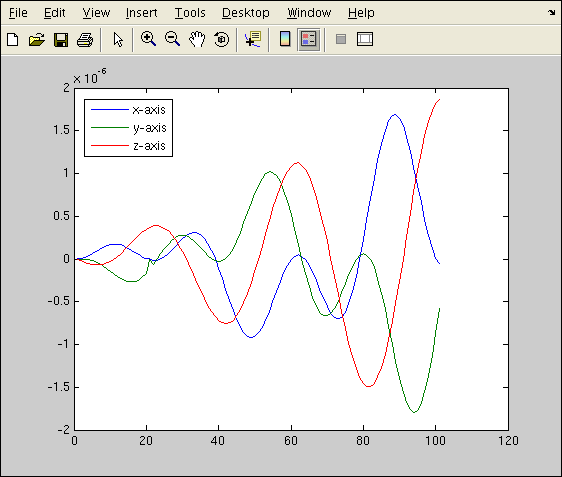
\includegraphics[width=80mm]{figures/relative6_xab.png}
        \caption{The variation with time of the difference between the analytical and numerical solutions for the position of A with respect to B.}
        \label{fig:rel6_1}
  \end{center}
\end{figure}

 \begin{figure}[!ht]
  \begin{center}
        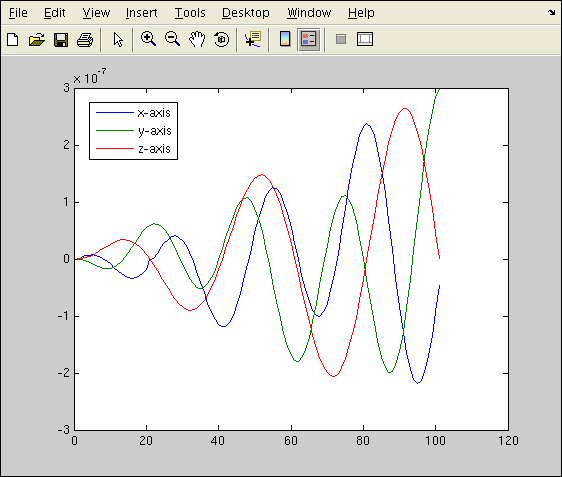
\includegraphics[width=80mm]{figures/relative6_vab.png}
        \caption{The variation with time of the difference between the analytical and numerical solutions for the velocity of A with respect to B.} 
  \end{center}
\end{figure}

 \begin{figure}[!ht]
  \begin{center}
        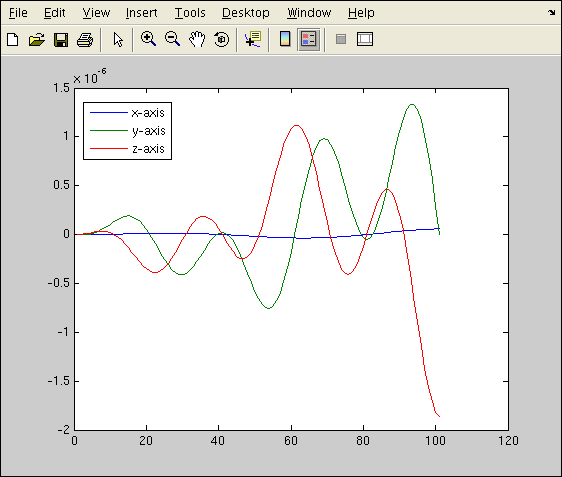
\includegraphics[width=80mm]{figures/relative6_xba.png}
        \caption{The variation with time of the difference between the analytical and numerical solutions for the position of B with respect to A.} 
  \end{center}
\end{figure}

 \begin{figure}[!ht]
  \begin{center}
        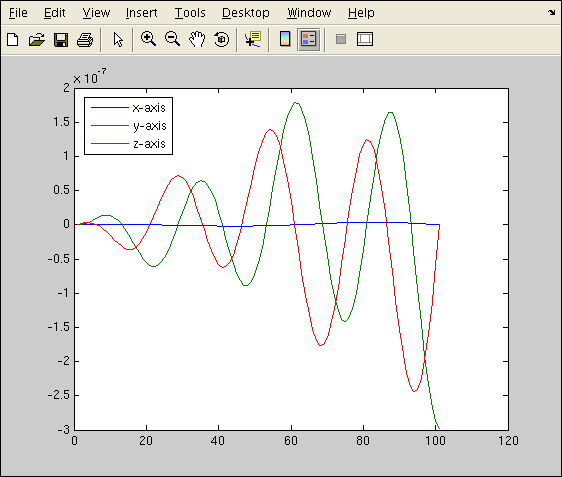
\includegraphics[width=80mm]{figures/relative6_vba.png}
        \caption{The variation with time of the difference between the analytical and numerical solutions for the velocity of B with respect to A.}
        \label{fig:rel6_4} 
  \end{center}
\end{figure}

 \begin{figure}[!ht]
  \begin{center}
        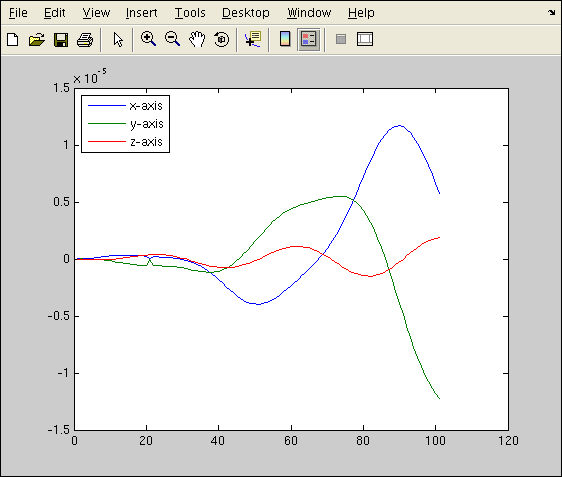
\includegraphics[width=80mm]{figures/relative7_xab.png}
        \caption{The variation with time of the difference between the analytical and numerical solutions for the position of A with respect to B.}
        \label{fig:rel7_1}
  \end{center}
\end{figure}

 \begin{figure}[!ht]
  \begin{center}
        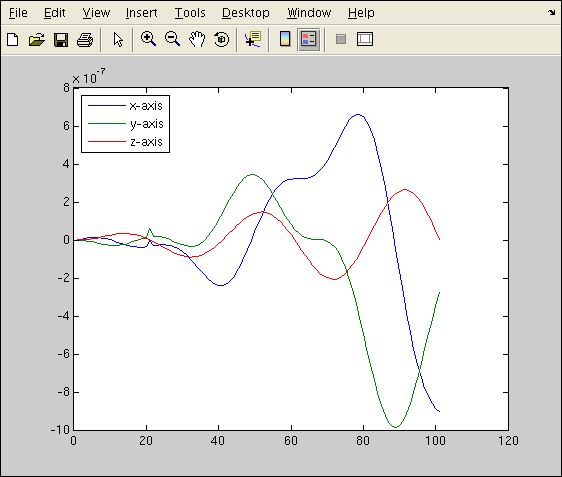
\includegraphics[width=80mm]{figures/relative7_vab.png}
        \caption{The variation with time of the difference between the analytical and numerical solutions for the velocity of A with respect to B.} 
  \end{center}
\end{figure}

 \begin{figure}[!ht]
  \begin{center}
        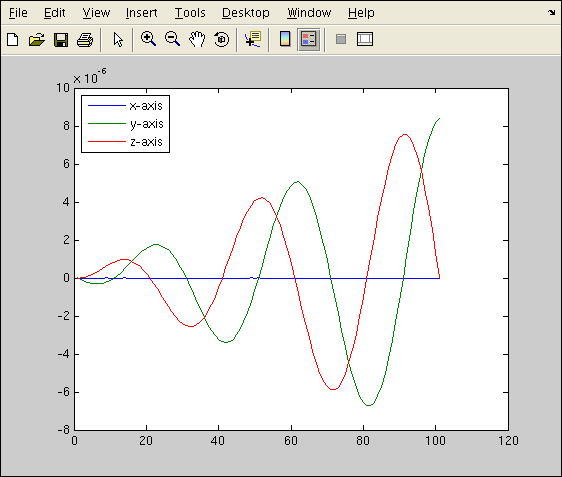
\includegraphics[width=80mm]{figures/relative7_wab.png}
        \caption{The variation with time of the difference between the analytical and numerical solutions for the angular velocity of A with respect to B.} 
  \end{center}
\end{figure}

\begin{figure}[!ht]
  \begin{center}
        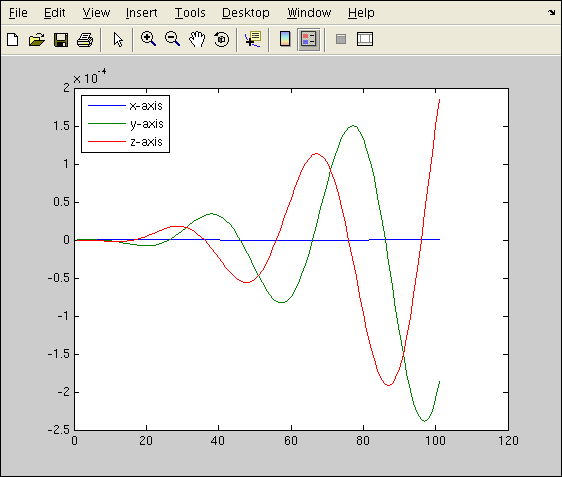
\includegraphics[width=80mm]{figures/relative7_xba.png}
        \caption{The variation with time of the difference between the analytical and numerical solutions for the position of B with respect to A.} 
  \end{center}
\end{figure}

 \begin{figure}[!ht]
  \begin{center}
        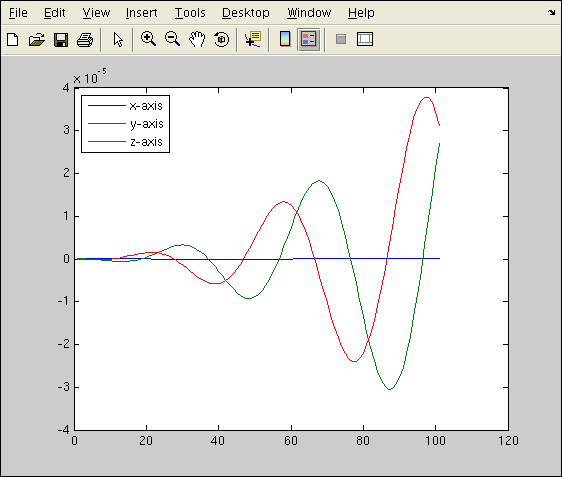
\includegraphics[width=80mm]{figures/relative7_vba.png}
        \caption{The variation with time of the difference between the analytical and numerical solutions for the velocity of B with respect to A.} 
  \end{center}
\end{figure}

\begin{figure}[!ht]
  \begin{center}
        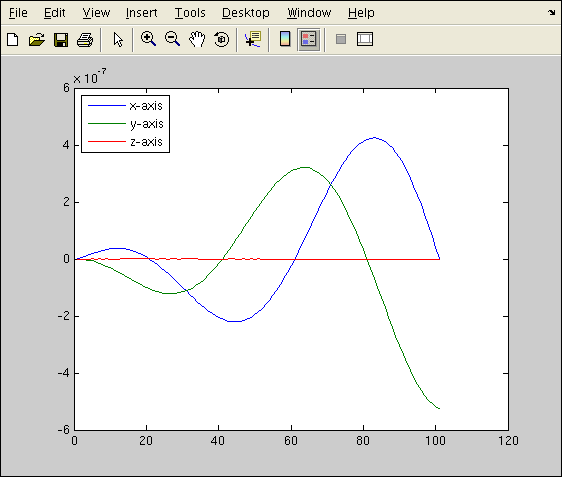
\includegraphics[width=80mm]{figures/relative7_wba.png}
        \caption{The variation with time of the difference between the analytical and numerical solutions for the angular velocity of B with respect to A.}
        \label{fig:rel7_6} 
  \end{center}
\end{figure}

\end{description}


%\section{Validation}
%%%%%%%%%%%%%%%%%%%%%%%%%%%%%%%%%%%%%%%%%%%%%%%%%%%%%%%%%%%%%%%%%%%%%%%%%%%%%%%%%
%
% Purpose:  Validation part of V&V for the Relative model
%
% 
%
%%%%%%%%%%%%%%%%%%%%%%%%%%%%%%%%%%%%%%%%%%%%%%%%%%%%%%%%%%%%%%%%%%%%%%%%%%%%%%%%

\section{Validation}

There is no independent validation of the \RelativeDesc.



